\section{Aufbau und Implementierung von Simulink-Blöcken}
Ein Simulink-Block muss Funktionen bereitstellen um die einzelnen Schritte einer Simulation zu ermöglichen. Darunter fallen die Folgenden Funktionen:

\begin{itemize}
	\item Initialisierung des Blocks
	\item Berechnung des nächsten Abtastzeitpunktes (falls der Block variable Abtastraten benötigt)
	\item Berechnung der Ausgangswerte
	\item Berechnung der diskreten Zustände des Blocks
	\item Integration, hierunter fallen die Berechnung der Ausgangswerte und Ableitungen bei Zwischenschritten (wird nur bei kontinuierlichen Zuständen benötigt)
\end{itemize}

Die Umsetzung dieser Methoden erfolgt in der Form einer sogenannten \textit{S-Function}. Hierbei handelt es sich lediglich um eine Sammlung von Funktionen, welche die oben genannten Aktionen implementieren. Eine \textit{S-Function} kann in unterschiedlichen Programmiersprachen implementiert werden, wobei MATLAB und C/C++ die üblichsten sind. Hier sollen lediglich \textit{S-Functions} in C/C++ vorgestellt werden, in \cite{SFunc} werden alle Alternativ detailliert erklärt. 

\subsection{C/C++ S-Function}
In diesem Abschnitt wird der Aufbau einer \textit{S-Function} am Beispiel eines einfachen Blocks, der seinen Eingang mit einem fixen Wert multipliziert, erklärt. Dieser Block benötigt keine kontinuierlichen Zustände, somit müssen lediglich Funktionen zur Initialisierung, Berechnung der Ausgänge und Terminierung am Ende der Simulation implementiert werden.

\begin{figure}[h]
\label{CustomGain_Overview_pic}
	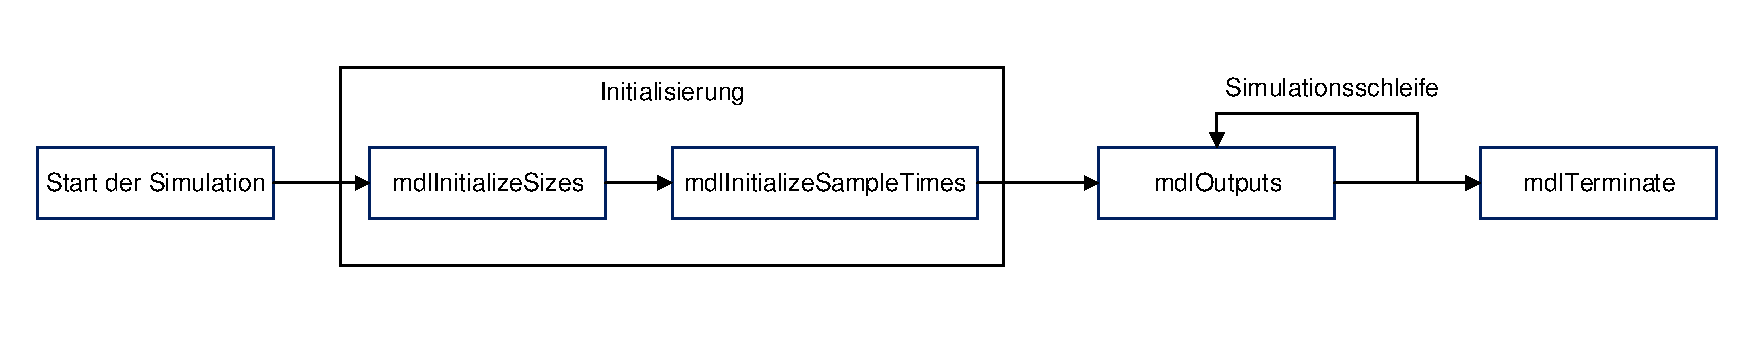
\includegraphics[width=\linewidth]{CustomGain_Overview}
	\caption{Interaktion eines diskreten Block mit der Simulink-Engine, Quelle: eigene Darstellung, Inhalt aus \cite{SFunc}}
\end{figure}

Die Implementierung in C++ beginnt mit der Definition der des Namen und Level der \textit{S-Function}. Das Level einer \textit{S-Function} sollte auf 2 gesetzt werden, bei dem Level 1 handelt es sich um einen veralteten \textit{S-Function} Typ. Außerdem werden die benötigten Header-Dateien inkludiert.

\begin{lstlisting}
#define S_FUNCTION_NAME CustomGain_SFunction
#define S_FUNCTION_LEVEL 2

#include "simstruc.h"
#include "matrix.h"
\end{lstlisting}

Anschließend werden die in \ref{CustomGain_Overview_pic} dargestellten Funktionen implementiert. Die Funktion \textit{mdlInitializeSizes} legt die Anzahl der Parameter, Ein- und Ausgänge fest. Anschließend werden die Weiten der Ein- bzw. Ausgangssignale eingestellt und die Anzahl der Abtastraten festgesetzt. Hierfür wird das s.g. \textit{SimStruct} verwendet. Hierbei handelt es sich um eine Baumstruktur, welche die Informationen über das gesamte Model und Blöcke enthält. Die Wurzel des \textit{SimStruct} ist das gesamt Modell, welches in die verschiedenen Subsysteme und Blöcke verzweigt. Die \textit{SimStruct}-Referenz die den Funktionen einer \textit{S-Function} übergeben wird, verweist auf das jeweilige Blatt der Baumstruktur, welche den Block repräsentiert.

\begin{lstlisting}
static void mdlInitializeSizes(SimStruct* S)
{
    //Anzahl der S-Function Parameter festlegen
    ssSetNumSFcnParams(S,1);         
    if(ssGetNumSFcnParams(S) != ssGetSFcnParamsCount(S)) return;
    
    //Anzahl der Eingaenge und deren Weite festlegen und ueberpruefen
    if(!ssSetNumInputPorts(S,1)) return;
    ssSetInputPortWidth(S, 0, 1);
    ssSetInputPortDirectFeedThrough(S, 0, 1);
    
    //Anzahl der Ausgaenge und deren Weite festlegen
    if(!ssSetNumOutputPorts(S,1)) return;
    ssSetOutputPortWidth(S, 0, DYNAMICALLY_SIZED);
    
    //Anzahl der Abtastsraten festlegen
    ssSetNumSampleTimes(S, 1);
}
\end{lstlisting}

In der Initialisierungsphase müssen außerdem die Abtastraten spezifiziert werden. Dies geschieht in der Funktion \textit{mdlInitializeSampleTimes}. Der Wert \textit{INHERITED\_SAMPLE\_TIME} bedeutet, dass die Abtastrate der Blöcke, welche das Ausgangssignal erhalten, übernommen wird.

\begin{lstlisting}
static void mdlInitializeSampleTimes(SimStruct* S)
{
    //Festelegen der Abtastrate und Abtastoffset auf INHERITED
    ssSetSampleTime(S, 0, INHERITED_SAMPLE_TIME);
    ssSetOffsetTime(S, 0, 0.0);
}
\end{lstlisting}

Während der Simulation ruft die Simulink-Engine die \textit{mdlOutputs} Funktion auf um den Ausgangswert des Blocks zu ermitteln. In diesem Fall wird der Eingangswert mit dem Block-Parameter multipliziert.

\begin{lstlisting}
static void mdlOutputs(SimStruct* S, int_T tid)
{   
    //Eingang-, Ausgangsignale und Parameter von dem SimStruct abfragen
    InputRealPtrsType inputPtrArr  = ssGetInputPortRealSignalPtrs(S, 0);
    real_T* outputPtr              = ssGetOutputPortRealSignal(S, 0);
    const mxArray* parameterPtr    = ssGetSFcnParam(S, 0);
    //Ausgangswert berechnen
    *outputPtr = (*(inputPtrArr[0])) * (*mxGetPr(parameterPtr));
}
\end{lstlisting}

Am Ende der Simulation wird die \textit{mdlTerminate} Funktion ausgeführt. Hier müssen ggf. reservierte Ressourcen wieder freigeben werden.

\begin{lstlisting}
static void mdlTerminate(SimStruct* S)
{
}
\end{lstlisting}

Am Schluss der C++-Datei befinden sich weitere Präprozessordirektiven, welche für die Codegeneration und MEX-Compilation benötigt werden. Diese beiden Ausführungsmodi werden in einem späteren Abschnitt näher erläutert.

\begin{lstlisting}
#ifdef MATLAB_MEX_FILE
#include "simulink.c"
#else
#include "cg_sfun.h"
#endif
\end{lstlisting}

\subsection{Codegeneration einer S-Function}
Eine \textit{S-Function} kann auch in Quellcode übersetzt werden. Die einfachste Form besteht in einer s.g. \textit{non-inlined S-Function}, die darin besteht, dass die C/C++-Datei der \textit{S-Function} direkt als Quelldatei verwendet wird. Somit muss allerdings das komplette \textit{SimStruct} in Quellcode übersetzt werden und den \textit{S-Function} während der Ausführung übergeben werden, wodurch die Größe und Ausführungszeit des Modelles erhöht wird. 

Mit Hilfe von TLC-Dateien kann eine \textit{S-Function} effizient in Quellcode übersetzt werden. In der TLC-Datei werden die Vorschriften festgehalten, wie die Ausgangswerte und Zustände eines Blocks in der gewählten Programmiersprache berechnet werden. Der folgende Codeausschnitt zeigt die \ac{TLC}-Implementation der bereits gezeigten Gain-\textit{S-Function}.

\begin{lstlisting}
%implements "CustomGain_SFunction" "C"

%function Outputs(block, system) Output
    %assign gainFactor  = LibBlockParameter(0, "", "", 0)
    %assign inputValue  = LibBlockInputSignal(0, "", "", 0)
    %assign outputValue = LibBlockOutputSignal(0, "", "", 0)
    %<outputValue>      = %<inputValue> * %<gainFactor>
%endfunction
\end{lstlisting}

Für den Quellcode muss lediglich die Output-Funktion generiert werden, in welcher das Eingangsignal mit dem Wert des Blockparameter multipliziert wird. Auf die Syntax und Funktionalität von \ac{TLC} wird hier nicht näher eingegangen, da Simulink mehrere Werkzeuge zur Verfügung stellt, die es ermöglichen \textit{S-Functions} und die zugehörigen TLC-Dateien automatisch zu erzeugen. Diese werden in den nächsten Abschnitt genauer erklärt.

\subsection{Kompilierung einer S-Function}
C/C++ \textit{S-Functions} müssen in MEX-Dateien übersetzt werden, damit sie in Simulink verwendet werden können. Matlab kann hierfür verschiedene Compiler wie z.B. \textit{MinGW} oder \textit{GCC} verwenden. Eine C/C++ Quelldatei kann über die Matlab Konsole mit dem folgenden Befehl in eine MEX-Datei übersetzt werden.

\begin{lstlisting}
mex CustomGain_SFunction.cpp
\end{lstlisting}

Matlab wählt hier automatisch den Compiler, welcher der Dateiendung entspricht. In dem Fall, das mehrere MEX-kompatible Compiler installiert sind, kann mit dem folgenden Befehl der gewünschte Compiler ausgewählt werden.

\begin{lstlisting}
mex -setup myCompiler
\end{lstlisting}

Die Verwendung von TLC-Dateien zur Codegeneration einer \textit{S-Function} bringt hier weitere Vorteile mit sich. Da eine \textit{non-inlined S-Function} ihre C/C++-Quelldatei sowohl für die MEX- als auch Target-Kompilierung verwendet wird, muss mit Hilfe von Makros der Quellcode geteilt werden. Der erste Teil dient als Quelle für die MEX-Datei. Der zweite Teil wird für die generierte Datei verwendet.

\begin{lstlisting}
#ifdef MATLAB_MEX_FILE
	/* Quellcode fuer die MEX-Datei */
#else
	/* Quellcode fuer die Zielplattform */
#endif
\end{lstlisting}

Dadurch ensteht eine unnötig große und unübersichtliche Quelldatei. Bei der Verwendung einer TLC-Datei wird die C/C++-Quelle lediglich für die MEX-Kompilierung verwendet. Der Quellcode für die Zielplattform-Kompilierung wird mit Hilfe der TLC-Datei kompiliert.

\subsection{S-Function-Builder}
Simulink bietet neben den gewöhnlichen \textit{S-Function}-Blöcken auch einen \textit{S-Function-Builder}-Block. Dieser bietet eine graphische Benutzeroberfläche, welche die Konfiguration einer \textit{S-Function} ermöglicht. Der \textit{S-Function-Builder} erzeugt im Anschluss eine C- und TLC-Datei und kompiliert die MEX-Datei. Dadurch kann die Entwicklung von Simulink-Blöcken stark vereinfacht werden, vor allem da keine TLC-Kenntnisse erforderlich sind.